\section{Direct sparse methods}
\label{subseq:sparse methods}

Direct sparse methods combine main advantages of direct and iterative methods i.e. numerical robustness and usage of sparsity structures. As a results, there is no need for preconditioning and the computation complexity is $O(n^2)$ \cite{complexity-of-spdm}. The problem is that storage cost can significantly increase during factorization i.e. the inverse of a sparse matrix can be sufficiently dense. To reduce storage space of $LU$ decomposition this group of methods performs fill-in reduction reodering as a pre-processing step before actual factorization. If storage space is still huge even after fill-in reduction reodering out-of core factorization can be used where partial results are stored in the secondary memory. \\

The most widely known sparse direct method is multifrontal method introduced by \citeauthor{mult-frontal-original:1} in their work \cite{mult-frontal-original:1}. Multifrontal method is an improved extension of a frontal method \cite{frontal-original} that can compute independent fronts in parallel. A front, or also called frontal matrix, can be considered as small dense matrix which is a result of Gaussian Elimination for a particular column. The algorithm, in fact, is as a variant of Gaussian Elimination process. There also exist left-looking and right-looking sparse direct methods. The difference between all of them is explained and can be found in \cite{elimination-tree}.\\


In order to understand and analyze strong scaling behavior of the algorithm we have to briefly discuss the theory of the multifrontal method. For simplicity we will assume that matrix $A$ is real symmetric and $LU$ decomposition boils down to the Cholesky factorization \ref{eq:chol-1}. It allows us to focus on the Cholesky factor $L$ and its sparsity pattern only.

\begin{equation} \label{eq:chol-1}
	A = LDL^T
\end{equation}

The algorithm usually starts with symbolic factorization to predict sparsity pattern of both $A$ and $L$. Once it is done a corresponding elimination tree has to be constructed.\\

\figpointer{\ref{fig:sparsity-pattern-example-mm}}

\begin{figure}[htpb]
  \centering
  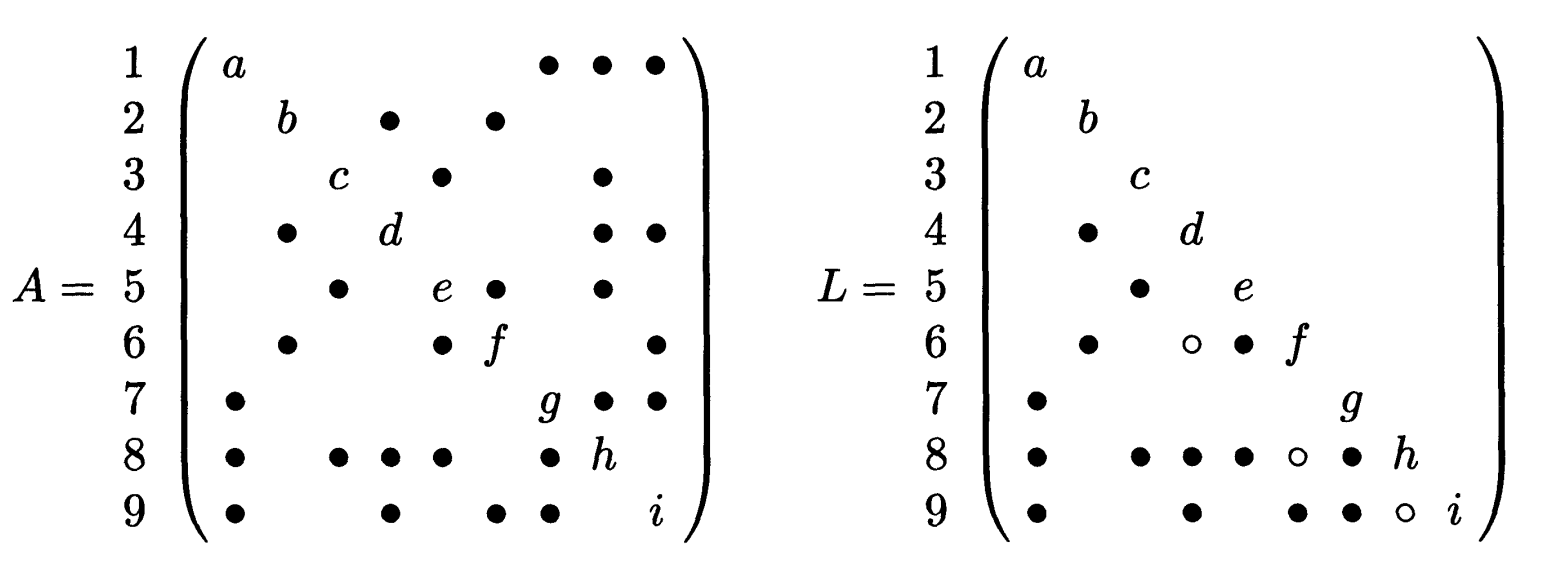
\includegraphics[width=0.9\textwidth]{figures/chapter-2/sparsity-pattern-example-mm.png}
\caption{An example of a sparse matrix and its Cholesky factor \cite{mult-frontal-original:2}}
\label{fig:sparsity-pattern-example-mm}
\end{figure}


Figure \ref{fig:sparsity-pattern-example-mm} shows an illustrative example of a sparse matrix and its Cholesky factor from \cite{mult-frontal-original:2}. The solid circles represent original non-zero elements whereas hollow ones define fill-in factors of $L$. \\


The elimination tree is a crucial part of the method. It can be considered as a structure of $n$ nodes that node $p$ is the parent of $j$ if and only if it satisfies equation \ref{eq:elimination-tree-1}. It is worth pointing out the definition \ref{eq:elimination-tree-1} is not only one possible and one can define a strucutre of an elimination tree in a different way as well. As an example one can find a definition of a general assembly tree in \cite{mult-frontal-original:2} proposed by \citeauthor{mult-frontal-original:2}.\\

\begin{equation} \label{eq:elimination-tree-1}
	p = min(i > j | l_{ij} \neq 0)
\end{equation}


It is important to notice that node $p$ represents elimination process of the corresponding column $p$ of matrix $A$ as well as all dependencies of column $p$ factorization on the results of its descendants.\\


Given definition \ref{eq:elimination-tree-1} we can build the corresponding elimination tree as it is shown in figure \ref{fig:elimination-tree-mm}.\\


\figpointer{\ref{fig:elimination-tree-mm}}

\begin{figure}[htpb]
  \centering
  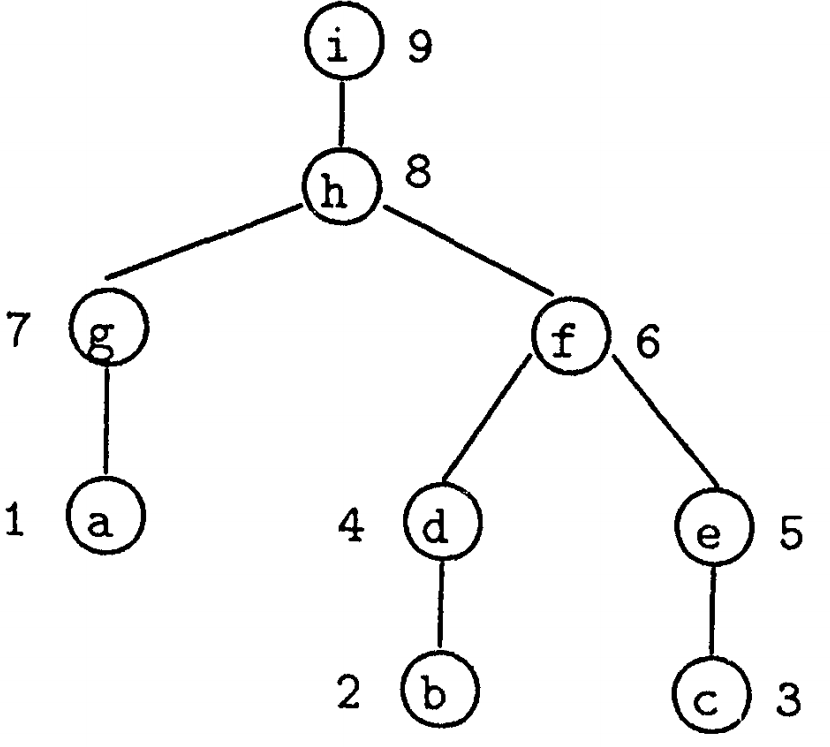
\includegraphics[width=0.45\textwidth]{figures/chapter-2/elimination-tree-mm.png}
\caption{The elimination tree for the matrix example in Figure \ref{fig:sparsity-pattern-example-mm}
 \cite{mult-frontal-original:2}}
\label{fig:elimination-tree-mm}
\end{figure}


The fundamental idea of multifrontal method spins around frontal and update matrices. A frontal matrix is used to perform Gaussian Elimination for a specific column $j$. It is a sum of a frame and update matrices as it can be seen from equation \ref{eq:mm-1}\\.

\begin{equation} \label{eq:mm-1}
	F_{j} = Fr_{j} + \hat{U_{j}} = \begin{bmatrix}a_{j,j} & a_{j,i_1} & a_{j,i_2} & \dots & a_{j,i_r} \\
a_{i_1,j} \\
a_{i_1,j} \\
\vdots & & & 0\\
a_{i_r,j} \\
\end{bmatrix} + \hat{U_{j}}
\end{equation}

where $i_{0}$, $i_{1}$, \dots , $i_{r}$ are the row subscripts of non-zeros in $L_{*j}$ with $i_{0} = j$ and $r$ is number of off-diagonal non-zero elements.\\

The frame matrix $Fr_{j}$ is filed with zeros except the first row and column. The first row and column contain non-zeros elements of the $j$th row and column of the original matrix $A$. Because we consider matrix $A$ to be symmetric the frame matrix is square and symmetric as well.\\

In order to describe parts of the elimination tree we will use the notation $T[j]$ to represent all descendants of the node $j$ in the tree and node $j$ itself. In this way we can define the update matrix $\hat{U_{j}}$ as following:\\

\begin{equation} \label{eq:mm-2}
	\hat{U_{j}} = - \sum_{k \in T[j] -{j}}  \begin{bmatrix}
l_{j,k} \\
l_{i_1,k} \\
\vdots \\
l_{i_1,k} \\
\end{bmatrix} \begin{bmatrix}
l_{j,k} & l_{i_1,k} & \dots & l_{i_1,k}
\end{bmatrix} 
\end{equation}


The update matrix $\hat{U_{j}}$ is, in fact, can be considered as the second term of the Schur complement i.e. update contributions from already factorized columns of $A$.\\

The subscript $k$ represents descendant columns of node $j$. Thus we include and consider only those elements of descendant columns which correspond to the non-zero pattern of the $j$th column that we are currently factorizing.\\

Let's consider the partial factorization of 2-by-2 block dense matrix to better understand essence of update matrix $\hat{U_{j}}$.\\


\begin{equation} \label{eq:mm-3}
A = \begin{bmatrix}
B & V^{T} \\
V & C
\end{bmatrix} 
= 
\begin{bmatrix}
L_{B} & 0 \\
VL^{-T}_{B} & I
\end{bmatrix}
\begin{bmatrix}
I & 0 \\
0 & C - VB^{-1}V^{T}
\end{bmatrix} 
\begin{bmatrix}
L^{T}_{B} & L^{-1}_{B}V^{T} \\
0 & I
\end{bmatrix} 
\end{equation}

Again we assume that $B$ has already been factorized and can be expressed as:

\begin{equation} \label{eq:mm-4}
	B = L_{B}L^{T}_{B}
\end{equation}

The Schur complement from equation \ref{eq:mm-3} can be viewed as the original sub-matrix $C$ and update $-VB^{-1}V^{T}$. It can be written in a vector form as well:

\begin{equation} \label{eq:mm-5}
	-VB^{-1}V^{T} = -(VL^{-T}_{B})(L^{-1}_{B}V^{T}) = - \sum_{k=1}^{j-1}  \begin{bmatrix}
l_{j,k} \\
\vdots \\
l_{n,k} \\
\end{bmatrix} \begin{bmatrix}
l_{j,k} & \dots & l_{n,k}
\end{bmatrix} 
\end{equation}

As it can be easily seen that equations \ref{eq:mm-5} and \ref{eq:mm-2} are identical. The difference is that equation \ref{eq:mm-2} exploits sparsity of the corresponding row and column of $L$ and thus masks unnecessary information. \\

% both eqautions show that the update matrix aggregate all previous information done and in case of the ,ultifrontal methods it means that we aggregate all information from descendants

% Therefore, we can express Uy as an aggregate of outer- product updates from columns in T[Cl],..., T[cs]. 

We can also notice from equation \ref{eq:mm-3} that the frame matrix $Fr_{j}$ corresponds to the block matrix $C$ and brings information from the original matrix $A$ whereas matrix $\hat{U_{j}}$ adds information about the columns that have already been factorized.\\

As soon as the frontal matrix $F_{j}$ is assembled i.e. we have complete update of column $j$, we can perform elimination of the first column and get non-zero entries of factor column $L_{*j}$.\\

Let's denote $\hat{F_{j}}$ as a result of the first column factorization of the frontal matrix $F_{j}$. Then we can express the results as following:\\


\begin{equation} \label{eq:mm-6}
\hat{F_{j}} = \begin{bmatrix}
l_{j,j} & \dots & 0 \\
\vdots & I \\
l_{i_{r},j} \\
\end{bmatrix} 
\begin{bmatrix}
1 & \dots & 0 \\
\vdots & U_{j} \\
0 \\
\end{bmatrix} 
\begin{bmatrix}
l_{j,j} & \dots & l_{i_{r},j} \\
\vdots & I \\
0 \\
\end{bmatrix} 
\end{equation}

where sub-matrix $U_{j}$ represents the full update from all descendants of node $j$ and node $j$ itself. Equation \ref{eq:mm-7} express the sub-matrix $U_{j}$ in a vector form.\\

\begin{equation} \label{eq:mm-7}
\hat{U_{j}} = - \sum_{k \in T[j]}  \begin{bmatrix}
l_{i_1,k} \\
\vdots \\
l_{i_1,k} \\
\end{bmatrix} \begin{bmatrix}
l_{i_1,k} & \dots & l_{i_1,k}
\end{bmatrix}
\end{equation}

Together with the frontal $F_{j}$ and update $\hat{U_j}$ matrices, the update column matrix $U_{j}$ forms the key concepts of the multifrontal method. To consider the importance of sub-matrix $U_{j}$ let's consider and example illustrated in Figure \ref{fig:information-float}.\\

\figpointer{\ref{fig:information-float}}
\begin{figure}[htpb]
  \centering
  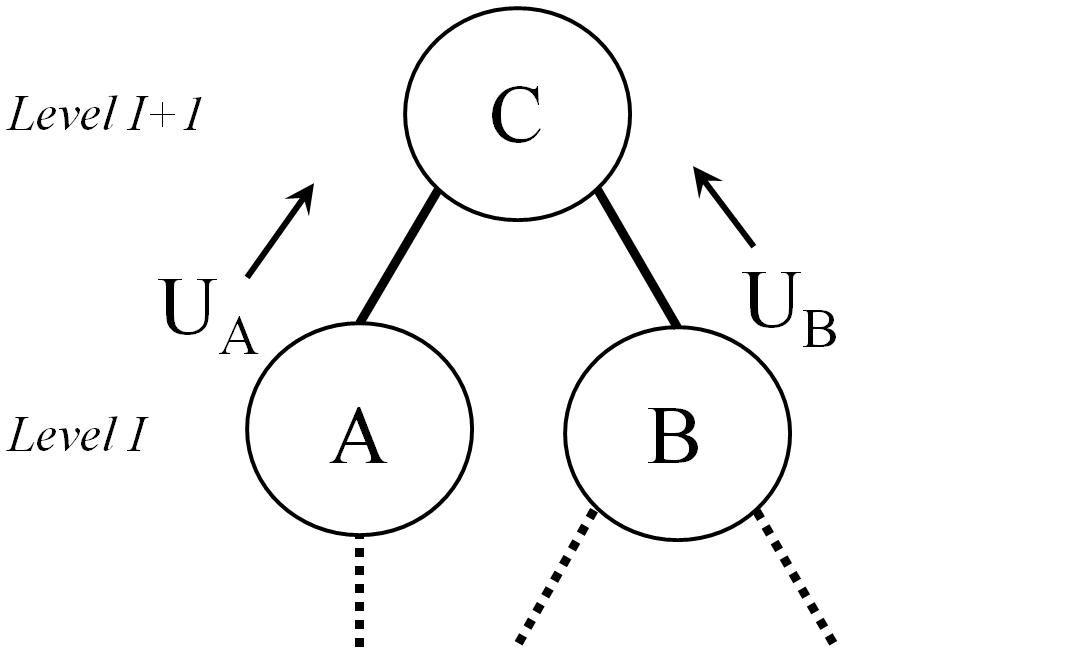
\includegraphics[width=0.45\textwidth]{figures/chapter-2/information-flow.png}
\caption{Information flow of the multifrontal method}
\label{fig:information-float}
\end{figure}


We assume that factorization of columns A and B have already been done and corresponding update column matrices $U_{A}$ and $U_{B}$ have been computed. From equation \ref{eq:mm-7} we have already known that both $U_{A}$ and $U_{B}$ contain the full updates of all their descendants including updates from factorization of columns $A$ and $B$. Therefore update column matrices $U_{A}$ and $U_{B}$ have already got all necessary information to construct update matrix $\hat{U_{C}}$. The detailed proof and careful explanation can be found in \cite{mult-frontal-original:2}.\\


It might happen that we do not need all rows and columns of $U_{A}$ and $U_{B}$ i.e. we need only some subset of them, because of sparsity of column $C$ . It is also important to place all necessary rows and columns of matrices $U_{A}$ and $U_{B}$ in a right place within matrix $\hat{U_{C}}$. For that reason, an additional matrix operation, called \textbf{\textit{extend-add}}, must be introduced.\\

Let's consider an example from \cite{mult-frontal-original:2} of an extend-add operation for 2-by-2 matrices $R$ and $S$ which correspond to the indices ${5,8}$ and ${5,9}$ of some matrix $B$, respectively.\\

\begin{equation}
R = \begin{bmatrix}
p & q \\
u & v \\
\end{bmatrix} 
,
\:
S = \begin{bmatrix}
w & x \\
y & z \\
\end{bmatrix} 
\end{equation}

The result of the operation is going to be a 3-by-3 $K$ matrix which looks as following:\\

\begin{equation} \label{eq:mm-8}
K = R \extendadd S = \begin{bmatrix}
p & q & 0 \\
u & v & 0 \\
0 & 0 & 0 \\
\end{bmatrix} 
+
\begin{bmatrix}
w & 0 & x \\
0 & 0 & 0 \\
y & 0 & z \\
\end{bmatrix} 
=
\begin{bmatrix}
p + w & q & x \\
u & v & 0 \\
y & 0 & z \\
\end{bmatrix} 
\end{equation}

Hence we can express formation of the frontal matrix $F_{j}$ using the extend-add operation and all direct children of node $j$ in the following way:


\begin{equation} \label{eq:mm-9}
	F_{j} = \begin{bmatrix}a_{j,j} & a_{j,i_1} & a_{j,i_2} & \dots & a_{j,i_r} \\
a_{i_1,j} \\
a_{i_1,j} \\
\vdots & & & 0\\
a_{i_r,j} \\
\end{bmatrix} \extendadd U_{c_1} \extendadd \dots \extendadd U_{c_s} 
\end{equation}

where $c_{1}, \: c_{2}, \: \dots \: c_{n}$ are indices of direct children of the node $j$.\\

Now it can be clearly seen that the resultant frontal matrix $F_{j}$ is a small dense one and it can be efficiently computed using BLAS level 3 subroutines.\\

After factorization we have to build complete column $j$ update matrix i.e. add columns and rows of $U_{c_1}, \:, U_{c_2}, \: \dots, U_{c_s}$ that have not been used in factorization of $F_{j}$ due to sparsity of column $j$. After that we can continue to move up along the tree. 
The complete update matrices grow in size as we move to the top of the tree. Therefore they have to be stored in a sparse matrix format to stay within memory constrains of the computer.\\


Up to this point we have already seen all key concepts of the multifrontal method and discussed how the algorithm works. We will move to the discussion of parallelization of the method. \\


The elimination tree, in fact, represents dependencies among columns. Conversely, the tree also shows independent and thus current steps of elimination process. Hence we can consider the tree as a source of task parallelism. For instance figure \ref{fig:elimination-tree-mm-parallel-steps} shows task parallelism where each color represents tasks that can be done in parallel.\\

\figpointer{\ref{fig:elimination-tree-mm-parallel-steps}}

\begin{figure}[htpb]
  \centering
  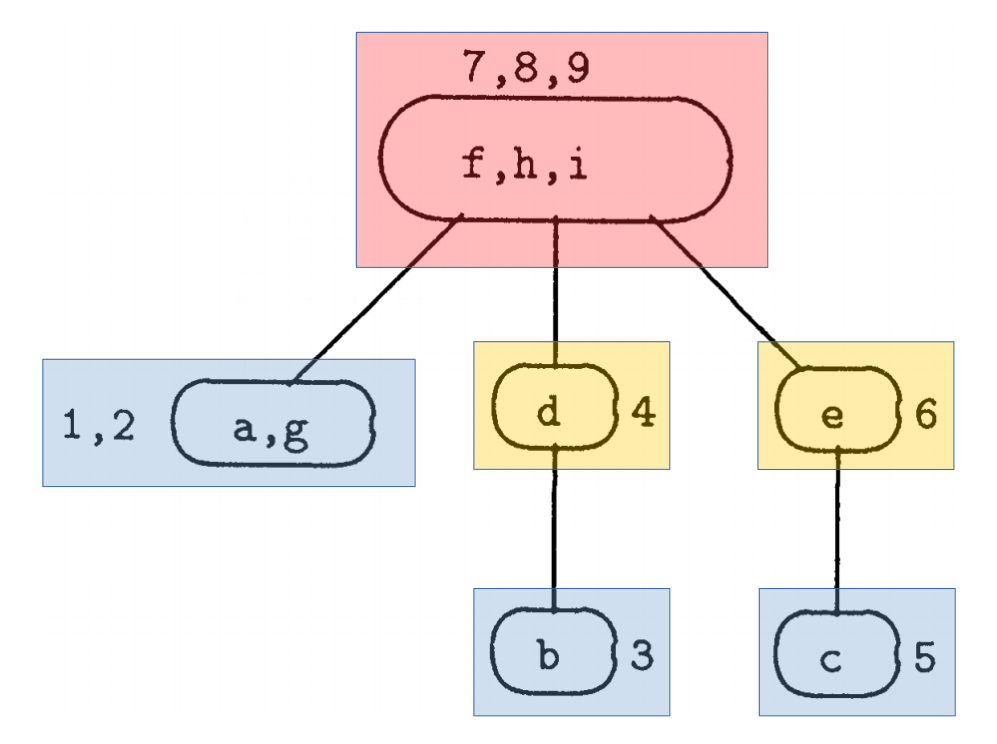
\includegraphics[width=0.45\textwidth]{figures/chapter-2/elimination-tree-parallel.png}
\caption{Parallel steps of the multifrontal method based on the example in Figures \ref{fig:sparsity-pattern-example-mm} and \ref{fig:elimination-tree-mm}}
\label{fig:elimination-tree-mm-parallel-steps}
\end{figure}


For example, nodes on separate branches of the tree are totally independent and can processed in parallel. However, as soon as at least two branches run into the same node it forms a dependency and we have to wait the complete update column matrices of its children and cannot proceed further.\\ 


We can observe the amount of task parallelism is rapidly decreasing while moving towards the root along the tree. Once we reach the root of the tree the algorithm becomes totally sequential. This fact plays the significant role in strong scaling behavior of the method.\\


We developed two simple models based on perfectly balanced binary trees to better understand strong scaling of the algorithm. The main concept of the models is so-called cost per level. This idea is similar to the recursion trees in \cite{recursion-tree} which explains and computes complexity of recurrent algorithms.\\

Let's assume 

\figpointer{\ref{fig:mm-parallel-model-tree}}

\begin{figure}[htpb]
 	\centering
	\begin{subfigure}[b]{0.65\textwidth}
		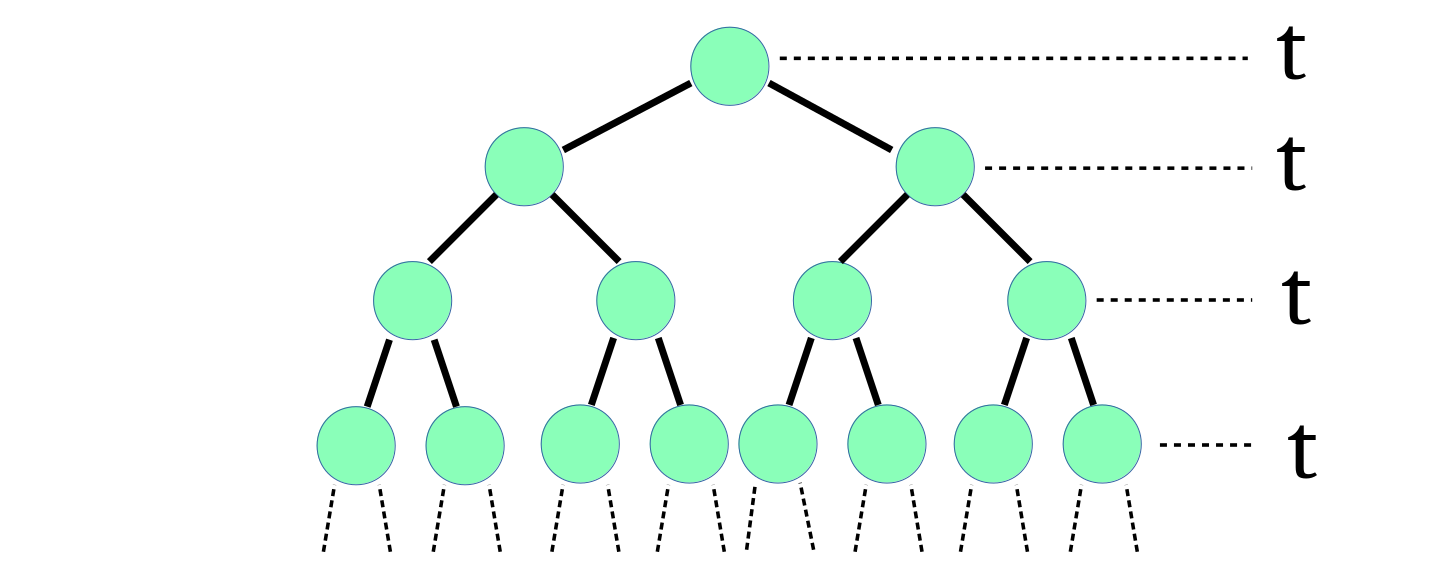
\includegraphics[width=1.0\textwidth]{figures/chapter-2/mm-parallel-model-tree-1.png}
		\caption{Model 1: equal cost per level}
	\end{subfigure}


	\begin{subfigure}[b]{0.65\textwidth}
		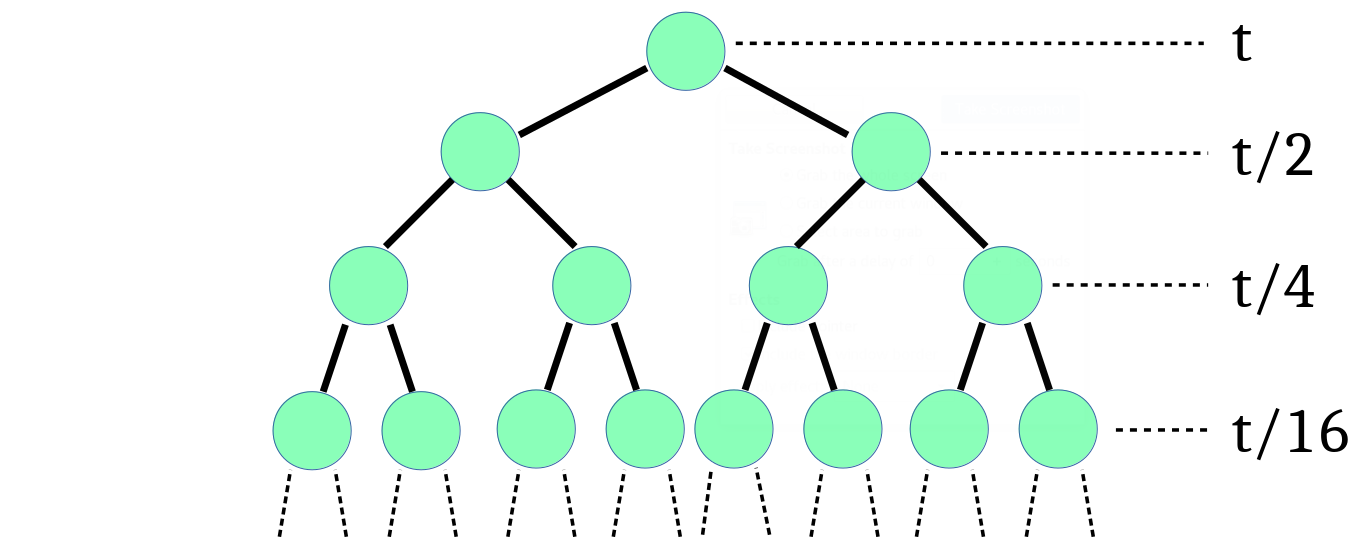
\includegraphics[width=1.0\textwidth]{figures/chapter-2/mm-parallel-model-tree-2.png}
		\caption{Model 2: quadratically decreasing cost per level}
	\end{subfigure}


  
\caption{Simple parallel models of the multifrontal method}
\label{fig:mm-parallel-model-tree}
\end{figure}


% Data parallelism


% carefull storage of olun update matrices  

 
 % additional tool



% storage strategy

% the importance of elimination trees can be found in []
% reference to the current paper 


%U contains all outer-productcontributions from columns in the subtree T[j]; while U contains those from columns in T[j] {j}.


% the second meaning of update matrices as an accumulator of information from previous steps


% consideration of small dense matrices

% which dense operations we use [unnecessary inria report]

% distribution of work load

% parallel model of the algorithm
















% to conclusion
There exist different implementations of multifrontal method on the market. Some implementations are open-source libraries (MUMPS, SuperLU, PaStiX, PSPASES, UMFPACK) and some of them are commercial packages (WSMP, PARDISO, etc.).
Some libraries can only handle Symmetric Positive Definite (SPD) matrices (PSPASES), some can run only sequentially (UMFPACK).\\

We can see from the primary documentations and literature review that MUMPS, PaStiX and SuperLU are open-source libraries and they can run on distributed environments in parallel. Both PaStiX and SuperLU are supernodal version of multifrontal method, whereas, MUMPS is the standard (classical) multifrontal implementation. [] showed in [] that MUMPS outperformed SuperLU \\






% a supernodal version of the multifrontal method where each node corresponds to the group of elements that make up a separator from the nested dissection method

% The factorization of the matrix is then organized by creating an elimination tree where each tree node is one of these supernodes. Sparse matrix factorization now becomes a series of factorizations of small dense blocks


% Give me the most popular sparce direct methods and compare them (goal: show that MUMPS it the most suitable package)
